\newpage
\thispagestyle{plain}
\vspace*{15cm} 
\begin{large}
\noindent
%\textbf{ACKNOWLEDGMENTS} \\
\textbf{POĎAKOVANIE} \\
\end{large}
\noindent
Chcem sa poďakovať môjmu vedúcemu Ing. Miroslavovi Blštákovi za odbornú pomoc, cenné rady, veľkú ochotu a nasmerovanie ma pri písaní práce. Taktiež sa chcem poďakovať ľudom, ktorí sa zúčastnili používateľského experimentu a všetkým, ktorí akokoľvek pomohli pri tvorbe tejto práce.
\newpage
\pagenumbering{gobble}
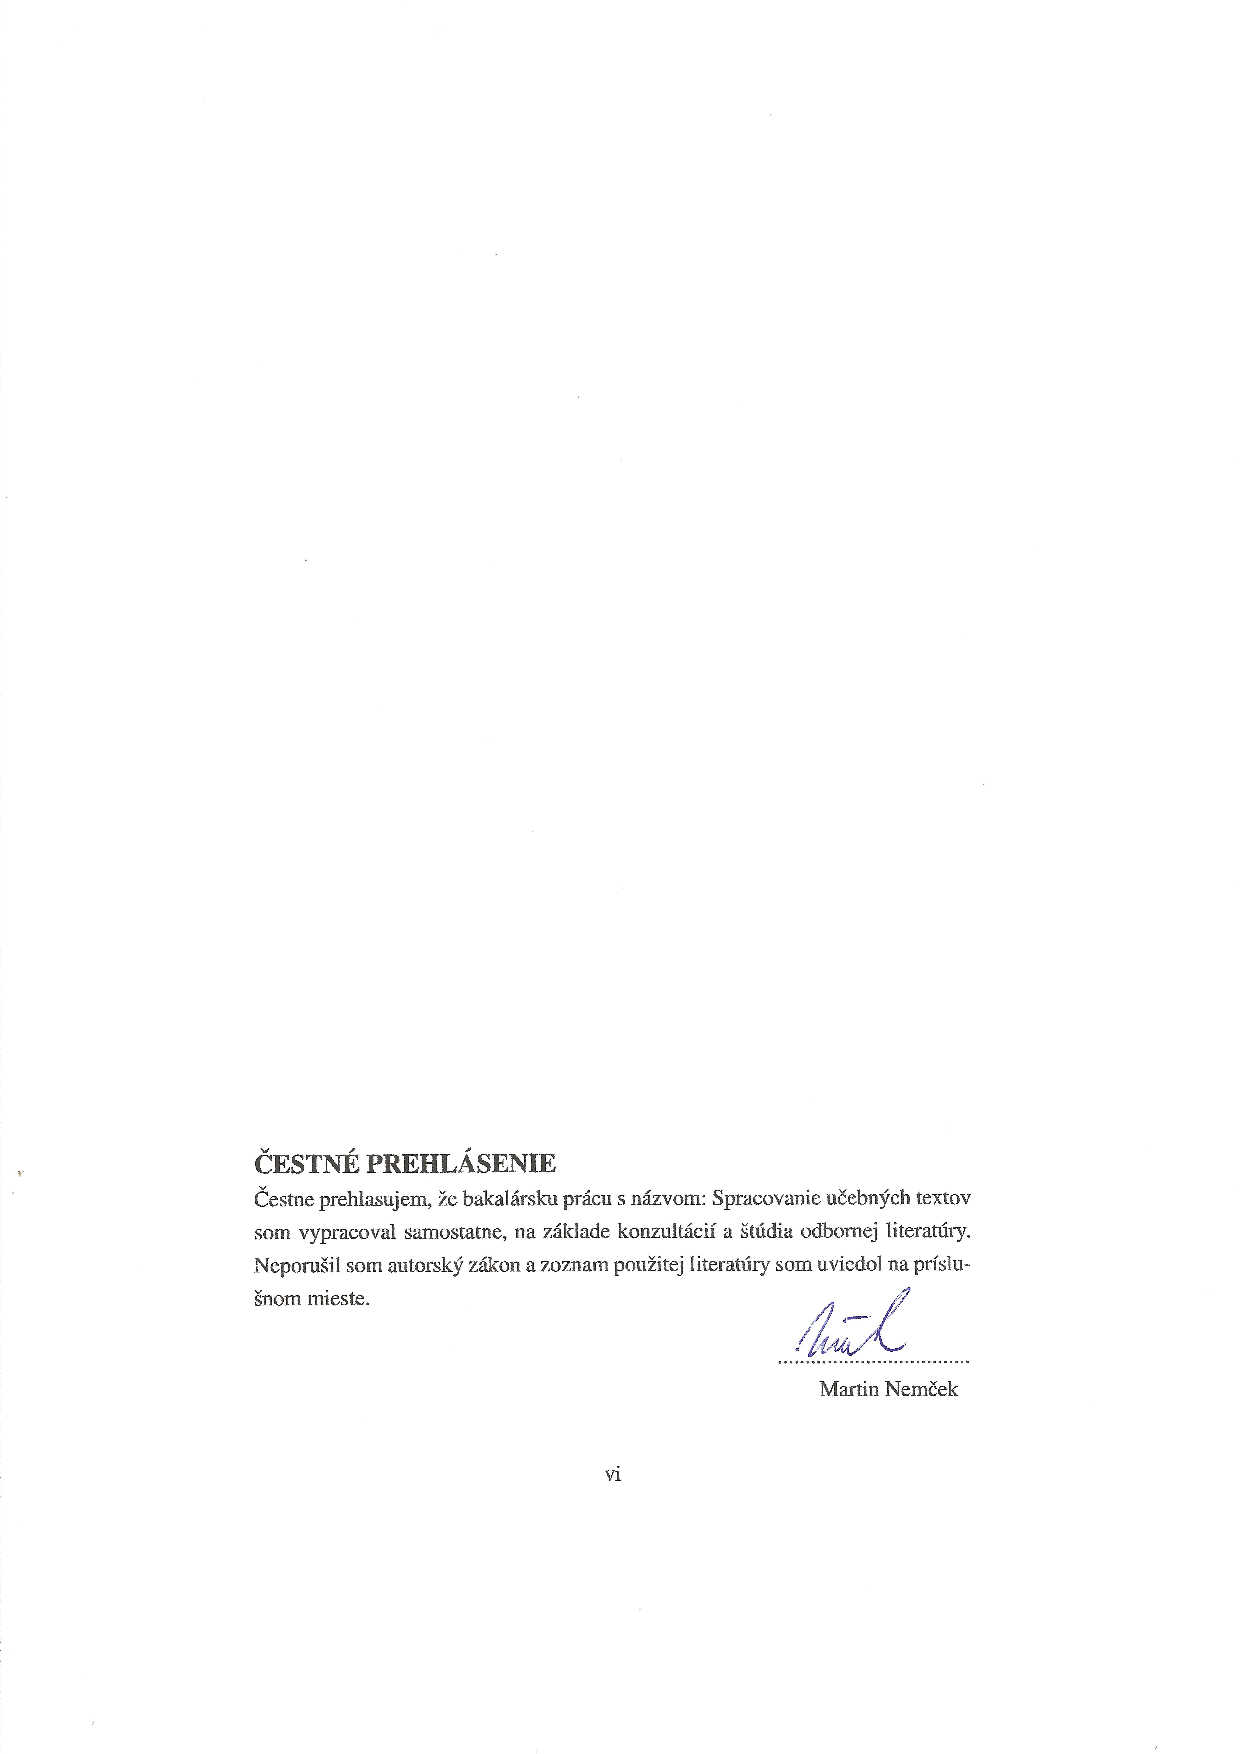
\includepdf[pages={1}, pagecommand={}]{declaration.pdf}
\pagenumbering{roman}\setcounter{page}{7}
%\thispagestyle{plain}
%\vspace*{15cm} 
%\begin{large}
%\noindent
%%\textbf{DECLARATION} \\
%\textbf{ČESTNÉ PREHLÁSENIE} \\
%\end{large}
%\noindent
%Čestne prehlasujem, že bakalársku prácu s názvom: Spracovanie učebných textov som vypracoval samostatne, na základe konzultácií a štúdia odbornej literatúry. Neporušil som autorský zákon a zoznam použitej literatúry som uviedol na príslušnom mieste.\vspace*{0.5cm}\\
%\hspace*{10cm}...................................\\
%\hspace*{10.7cm} \Author